% !TeX root = ../main.tex
%
\chapter{State Estimation}

Kalman filter top

quantization model
\begin{align}
x_q = \Delta \left\lfloor\ \frac{x}{\Delta} + \frac{1}{2}\ \right\rfloor \ \ \ ,   \label{eq:quantizationModel}
\end{align}

for x $\Delta_x =\ $\SI{0.088e-3} m/tic\\
with $\Delta_\theta =\ $\SI{\pi e-3} rad/tic and applying the quantization model to a smoothed version of the original measured signal is seen in \autoref{fig:quantizationProblem}.

\begin{figure}[H]
  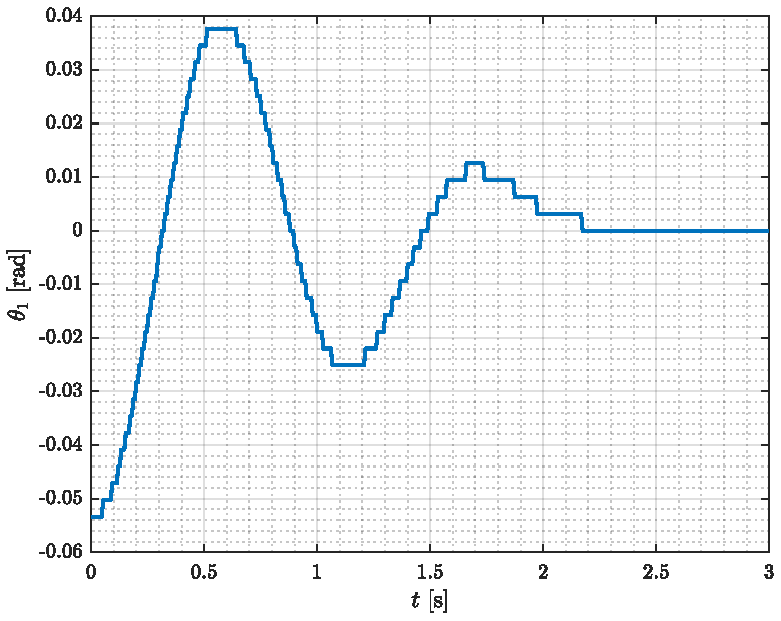
\includegraphics[width=.7\textwidth]{figures/quantizationProblem}
  \caption{a}
  \label{fig:quantizationProblem}
\end{figure}


Model
\begin{alignat}{3}
\vec{x}_{k} &= \vec{F} \vec{x}_{k-1} + \vec{G} u_{k-1} + \vec{w}_{k-1}  \ \ , &&\ \ \ \ \vec{w} \sim \mathcal{N}(0,\,\vec{Q})\,   \\
\vec{y}_k &= \vec{H} \vec{x}_k + \vec{v}_k                              \ \ , &&\ \ \ \ \vec{v} \sim \mathcal{N}(0,\,\vec{R})\,  \ \ \ , 
  \label{eq:discreteModelForKF}
\end{alignat}


\subsubsection{Initialization}
The previous predicted state vector, $\hat{\vec{x}}_{k-1}$ is initialized to the current measurements $y_k$,
%
\begin{align}
\hat{\vec{x}}_{k-1} &= y_k \ \ \ ,   \label{eq:xInit}
\end{align}
%
and the previous state error covariance $\vec{P}_{k-1}$ is initialized to some initial guess $\vec{P}_0$ here set to the identity matrix,
\begin{align}
\vec{P}_{k-1} &= \vec{P}_0  \ \ \ . \label{eq:initP}
\end{align}
%
When the Kalman filter is running $\vec{P}$ will converge to some steady state values which is then be used as $\vec{P}_0$ in the implementation for faster convergence.

\subsubsection{Prediction}
\begin{align}
\hat{\vec{x}}_{k|k-1} &= \vec{F} \hat{\vec{x}}_{k-1} + \vec{G} u_{k-1} \ \ \ . \label{eq:predictedState}
\end{align}
%
\begin{align}
\vec{P}_{k|k-1} &= \vec{F} P_{k-1} \vec{F}^\mathrm{T} + \vec{Q}  \ \ \ . \label{eq:predictedStateErrorCovariance}
\end{align}
%
$k|k-1$ reads "$k$ given $k-1$".

\subsubsection{Update}
\begin{align}
\vec{K}_k &= \vec{P}_{k|k-1} \vec{H}^\mathrm{T} ( \vec{H} \vec{P}_{k|k-1} \vec{H}^\mathrm{T} + \vec{R} )^{-1}  \ \ \ . \label{eq:kalmanGain}
\end{align}
%
\begin{align}
\hat{\vec{x}}_k &= \hat{\vec{x}}_{k-1} + \vec{K}_k ( y_k - \vec{H} \hat{\vec{x}}_{k-1} ) \ \ \ . \label{eq:estimatedState}
\end{align}
where $\vec{H} \hat{\vec{x}}_{k-1} = \hat{\vec{y}}_{k-1}$ is the predicted output.
%
\begin{align}
\vec{P}_k &= ( \vec{I} - \vec{K}_k \vec{H} ) \vec{P}_{k|k-1} \ \ \ . \label{eq:stateErrorCovariance}
\end{align}

The measurement noise covariance is tuned such that the quantization problem is solved, see \autoref{fig:theta1_KFsim},
\begin{align}
\vec{R} &= diag( 100,\ 100,\ 10 )  \ \ \ .
\end{align}
%
\begin{figure}[H]
  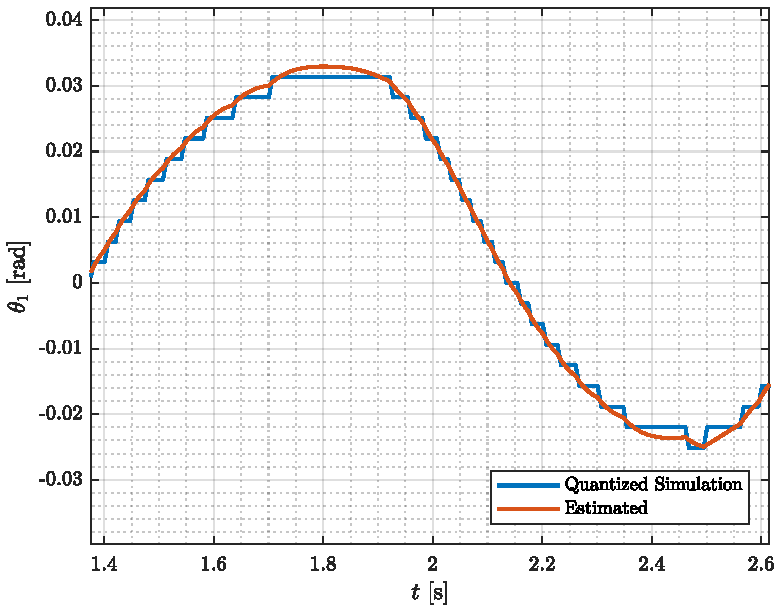
\includegraphics[width=.7\textwidth]{figures/theta1_KFsim}
  \caption{a}
  \label{fig:theta1_KFsim}
\end{figure}
%
The process noise covariance matrix is tuned to get as true estimations of the drivatives as possible while maintaining low noise levels,
\begin{align}
\vec{Q} &= diag( 1,\ 1,\ 1,\ 100,\ 100,\ 10 )  \ \ \ ,
\end{align}
see simulation in \autoref{fig:theta1Dot_KFsim}.
%
\begin{figure}[H]
  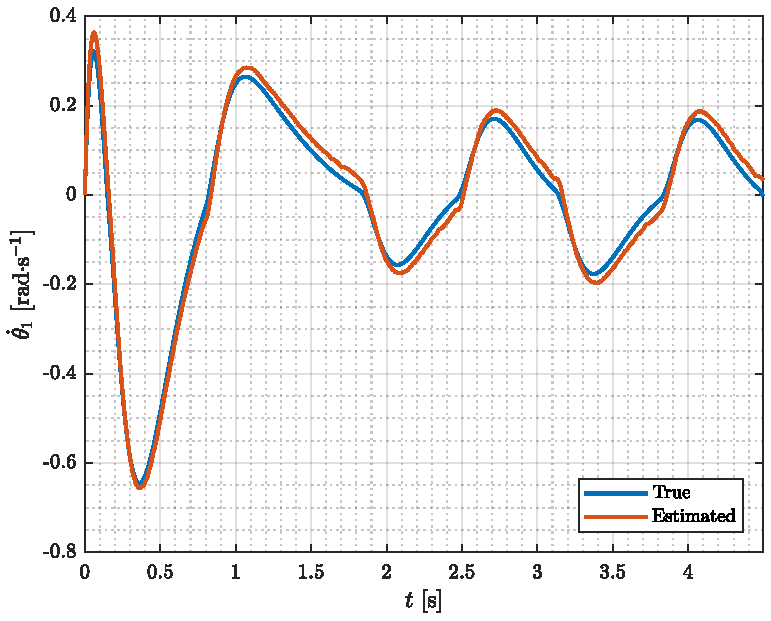
\includegraphics[width=.7\textwidth]{figures/theta1Dot_KFsim}
  \caption{a}
  \label{fig:theta1Dot_KFsim}
\end{figure}
%
Very similar results are obtained for the second pendulum. Since the quantization problem is more than an order of magnitude smaller for the position measurements compared to the angle measurements, the filter obtains near perfect results in simulation, see \autoref{fig:x_KFsim} and \ref{fig:xDot_KFsim}.
%
\begin{figure}[H]
  \hspace{-10pt}
  \captionbox
  {
    a
    \label{fig:x_KFsim}
  }
  {
    \hspace{-1cm}
    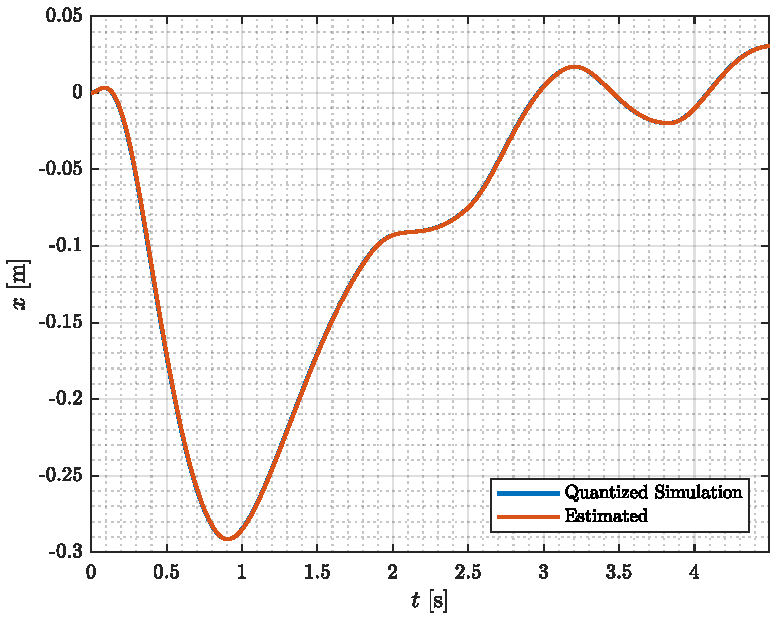
\includegraphics[width=.5\textwidth]{figures/x_KFsim}
  }
  \hspace{20pt}
  \captionbox 
  {
    a
    \label{fig:xDot_KFsim}
  }
  {
    \hspace{-1cm}
    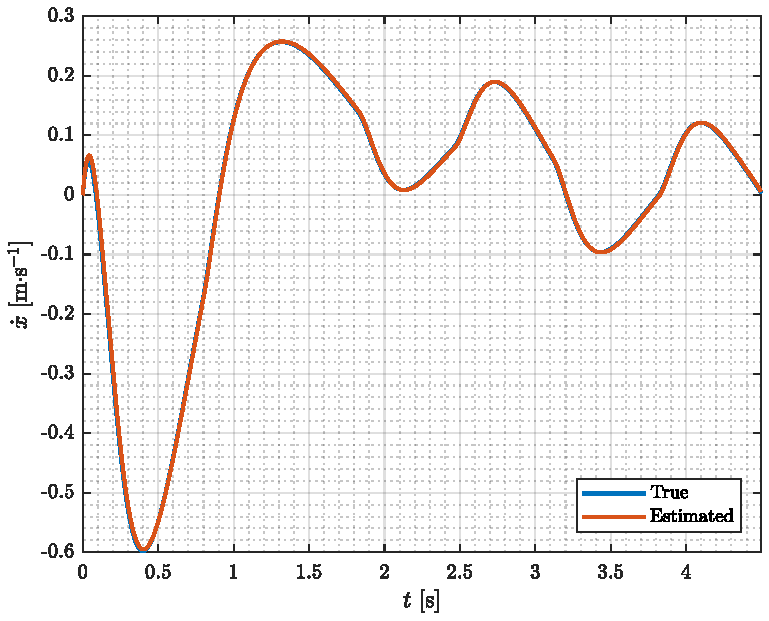
\includegraphics[width=.5\textwidth]{figures/xDot_KFsim}
  }  
\end{figure}
%
%other available plots
% theta2_KFsim
% theta2Dot_KFsim
%




%-------plots-----------

%  implemented Kalman filter













